\documentclass{standalone}
\usepackage{tikz}
\usetikzlibrary{patterns, positioning}

\begin{document}
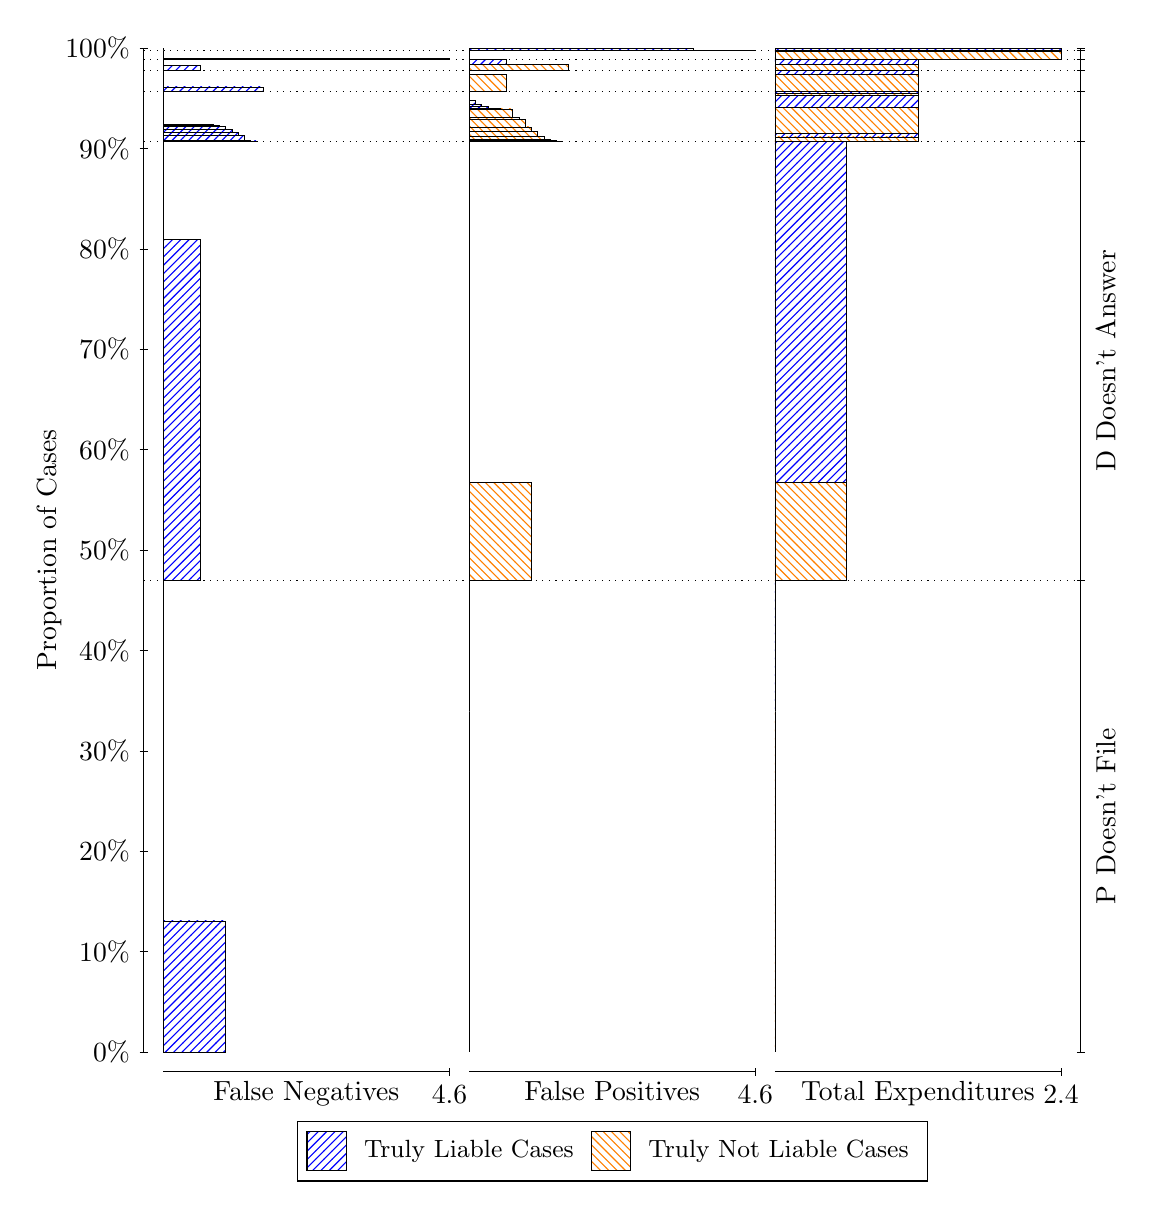
\begin{tikzpicture}
\draw[black, very thin] (1.5,1.75) -- (1.5,14.5);
\node[rotate=90, anchor=center] at (0.3, 8.125) {Proportion of Cases};
\draw[black, very thin] (1.45,1.75) -- (1.55,1.75);
\node[anchor=east] at (1.45, 1.75) {0\%};
\draw[black, very thin] (1.45,3.025) -- (1.55,3.025);
\node[anchor=east] at (1.45, 3.025) {10\%};
\draw[black, very thin] (1.45,4.3) -- (1.55,4.3);
\node[anchor=east] at (1.45, 4.3) {20\%};
\draw[black, very thin] (1.45,5.575) -- (1.55,5.575);
\node[anchor=east] at (1.45, 5.575) {30\%};
\draw[black, very thin] (1.45,6.85) -- (1.55,6.85);
\node[anchor=east] at (1.45, 6.85) {40\%};
\draw[black, very thin] (1.45,8.125) -- (1.55,8.125);
\node[anchor=east] at (1.45, 8.125) {50\%};
\draw[black, very thin] (1.45,9.4) -- (1.55,9.4);
\node[anchor=east] at (1.45, 9.4) {60\%};
\draw[black, very thin] (1.45,10.675) -- (1.55,10.675);
\node[anchor=east] at (1.45, 10.675) {70\%};
\draw[black, very thin] (1.45,11.95) -- (1.55,11.95);
\node[anchor=east] at (1.45, 11.95) {80\%};
\draw[black, very thin] (1.45,13.225) -- (1.55,13.225);
\node[anchor=east] at (1.45, 13.225) {90\%};
\draw[black, very thin] (1.45,14.5) -- (1.55,14.5);
\node[anchor=east] at (1.45, 14.5) {100\%};

\draw[black, very thin] (13.4,1.75) -- (13.4,14.5);
\draw[black, very thin] (13.35,1.75) -- (13.45,1.75);
\node[anchor=west] at (13.35, 1.75) {};
\draw[black, very thin] (13.35,7.7412) -- (13.45,7.7412);
\node[anchor=west] at (13.35, 7.7412) {};
\draw[black, very thin] (13.35,13.311) -- (13.45,13.311);
\node[anchor=west] at (13.35, 13.311) {};
\draw[black, very thin] (13.35,13.95) -- (13.45,13.95);
\node[anchor=west] at (13.35, 13.95) {};
\draw[black, very thin] (13.35,14.22) -- (13.45,14.22);
\node[anchor=west] at (13.35, 14.22) {};
\draw[black, very thin] (13.35,14.355) -- (13.45,14.355);
\node[anchor=west] at (13.35, 14.355) {};
\draw[black, very thin] (13.35,14.47) -- (13.45,14.47);
\node[anchor=west] at (13.35, 14.47) {};
\draw[black, very thin] (13.35,14.5) -- (13.45,14.5);
\node[anchor=west] at (13.35, 14.5) {};

\draw[black, very thin, pattern color=blue, pattern=north east lines] (1.75,1.75) rectangle (2.5399,3.4161);
\draw[black, very thin, pattern color=orange, pattern=north west lines] (1.75,3.4161) rectangle (1.75,7.7412);
\draw[black, very thin, pattern color=blue, pattern=north east lines] (1.75,7.7412) rectangle (2.2239,12.07);
\draw[black, very thin, pattern color=orange, pattern=north west lines] (1.75,12.07) rectangle (1.75,13.311);
\draw[black, very thin, pattern color=blue, pattern=north east lines] (1.75,13.311) rectangle (2.9348,13.32);
\draw[black, very thin, pattern color=blue, pattern=north east lines] (1.75,13.32) rectangle (2.8558,13.331);
\draw[black, very thin, pattern color=blue, pattern=north east lines] (1.75,13.331) rectangle (2.7768,13.387);
\draw[black, very thin, pattern color=blue, pattern=north east lines] (1.75,13.387) rectangle (2.6978,13.425);
\draw[black, very thin, pattern color=blue, pattern=north east lines] (1.75,13.425) rectangle (2.6188,13.47);
\draw[black, very thin, pattern color=blue, pattern=north east lines] (1.75,13.47) rectangle (2.5399,13.5);
\draw[black, very thin, pattern color=blue, pattern=north east lines] (1.75,13.5) rectangle (2.4609,13.521);
\draw[black, very thin, pattern color=blue, pattern=north east lines] (1.75,13.521) rectangle (2.3819,13.529);
\draw[black, very thin, pattern color=blue, pattern=north east lines] (1.75,13.529) rectangle (2.3029,13.534);
\draw[black, very thin, pattern color=orange, pattern=north west lines] (1.75,13.534) rectangle (1.75,13.95);
\draw[black, very thin, pattern color=blue, pattern=north east lines] (1.75,13.95) rectangle (3.0138,14.007);
\draw[black, very thin, pattern color=orange, pattern=north west lines] (1.75,14.007) rectangle (1.75,14.22);
\draw[black, very thin, pattern color=blue, pattern=north east lines] (1.75,14.22) rectangle (2.2239,14.284);
\draw[black, very thin, pattern color=orange, pattern=north west lines] (1.75,14.284) rectangle (1.75,14.355);
\draw[black, very thin, pattern color=blue, pattern=north east lines] (1.75,14.355) rectangle (5.3833,14.364);
\draw[black, very thin, pattern color=orange, pattern=north west lines] (1.75,14.364) rectangle (1.75,14.47);
\draw[black, very thin, pattern color=orange, pattern=north west lines] (1.75,14.47) rectangle (1.75,14.473);
\draw[black, very thin, pattern color=blue, pattern=north east lines] (1.75,14.473) rectangle (1.75,14.5);
\draw[black, very thin, pattern color=orange, pattern=north west lines] (5.6333,1.75) rectangle (5.6333,6.0751);
\draw[black, very thin, pattern color=blue, pattern=north east lines] (5.6333,6.0751) rectangle (5.6333,7.7412);
\draw[black, very thin, pattern color=orange, pattern=north west lines] (5.6333,7.7412) rectangle (6.4232,8.9822);
\draw[black, very thin, pattern color=blue, pattern=north east lines] (5.6333,8.9822) rectangle (5.6333,13.311);
\draw[black, very thin, pattern color=orange, pattern=north west lines] (5.6333,13.311) rectangle (6.8181,13.317);
\draw[black, very thin, pattern color=orange, pattern=north west lines] (5.6333,13.317) rectangle (6.7391,13.323);
\draw[black, very thin, pattern color=orange, pattern=north west lines] (5.6333,13.323) rectangle (6.6601,13.342);
\draw[black, very thin, pattern color=orange, pattern=north west lines] (5.6333,13.342) rectangle (6.5812,13.377);
\draw[black, very thin, pattern color=orange, pattern=north west lines] (5.6333,13.377) rectangle (6.5022,13.439);
\draw[black, very thin, pattern color=orange, pattern=north west lines] (5.6333,13.439) rectangle (6.4232,13.499);
\draw[black, very thin, pattern color=orange, pattern=north west lines] (5.6333,13.499) rectangle (6.3442,13.592);
\draw[black, very thin, pattern color=orange, pattern=north west lines] (5.6333,13.592) rectangle (6.2652,13.623);
\draw[black, very thin, pattern color=orange, pattern=north west lines] (5.6333,13.623) rectangle (6.1862,13.726);
\draw[black, very thin, pattern color=blue, pattern=north east lines] (5.6333,13.726) rectangle (6.0283,13.731);
\draw[black, very thin, pattern color=blue, pattern=north east lines] (5.6333,13.731) rectangle (5.9493,13.74);
\draw[black, very thin, pattern color=blue, pattern=north east lines] (5.6333,13.74) rectangle (5.8703,13.761);
\draw[black, very thin, pattern color=blue, pattern=north east lines] (5.6333,13.761) rectangle (5.7913,13.791);
\draw[black, very thin, pattern color=blue, pattern=north east lines] (5.6333,13.791) rectangle (5.7123,13.835);
\draw[black, very thin, pattern color=blue, pattern=north east lines] (5.6333,13.835) rectangle (5.6333,13.95);
\draw[black, very thin, pattern color=orange, pattern=north west lines] (5.6333,13.95) rectangle (6.1072,14.163);
\draw[black, very thin, pattern color=blue, pattern=north east lines] (5.6333,14.163) rectangle (5.6333,14.22);
\draw[black, very thin, pattern color=orange, pattern=north west lines] (5.6333,14.22) rectangle (6.8971,14.292);
\draw[black, very thin, pattern color=blue, pattern=north east lines] (5.6333,14.292) rectangle (6.1072,14.355);
\draw[black, very thin, pattern color=orange, pattern=north west lines] (5.6333,14.355) rectangle (5.6333,14.461);
\draw[black, very thin, pattern color=blue, pattern=north east lines] (5.6333,14.461) rectangle (5.6333,14.47);
\draw[black, very thin, pattern color=orange, pattern=north west lines] (5.6333,14.47) rectangle (9.2667,14.473);
\draw[black, very thin, pattern color=blue, pattern=north east lines] (5.6333,14.473) rectangle (8.4768,14.5);
\draw[black, very thin, pattern color=orange, pattern=north west lines] (9.5167,1.75) rectangle (9.5167,6.0751);
\draw[black, very thin, pattern color=blue, pattern=north east lines] (9.5167,6.0751) rectangle (9.5167,7.7412);
\draw[black, very thin, pattern color=orange, pattern=north west lines] (9.5167,7.7412) rectangle (10.425,8.9822);
\draw[black, very thin, pattern color=blue, pattern=north east lines] (9.5167,8.9822) rectangle (10.425,13.311);
\draw[black, very thin, pattern color=orange, pattern=north west lines] (9.5167,13.311) rectangle (11.333,13.372);
\draw[black, very thin, pattern color=blue, pattern=north east lines] (9.5167,13.372) rectangle (11.333,13.417);
\draw[black, very thin, pattern color=orange, pattern=north west lines] (9.5167,13.417) rectangle (11.333,13.745);
\draw[black, very thin, pattern color=blue, pattern=north east lines] (9.5167,13.745) rectangle (11.333,13.895);
\draw[black, very thin, pattern color=orange, pattern=north west lines] (9.5167,13.895) rectangle (11.333,13.92);
\draw[black, very thin, pattern color=blue, pattern=north east lines] (9.5167,13.92) rectangle (11.333,13.95);
\draw[black, very thin, pattern color=orange, pattern=north west lines] (9.5167,13.95) rectangle (11.333,14.163);
\draw[black, very thin, pattern color=blue, pattern=north east lines] (9.5167,14.163) rectangle (11.333,14.22);
\draw[black, very thin, pattern color=orange, pattern=north west lines] (9.5167,14.22) rectangle (11.333,14.292);
\draw[black, very thin, pattern color=blue, pattern=north east lines] (9.5167,14.292) rectangle (11.333,14.355);
\draw[black, very thin, pattern color=orange, pattern=north west lines] (9.5167,14.355) rectangle (13.15,14.461);
\draw[black, very thin, pattern color=blue, pattern=north east lines] (9.5167,14.461) rectangle (13.15,14.47);
\draw[black, very thin, pattern color=orange, pattern=north west lines] (9.5167,14.47) rectangle (13.15,14.473);
\draw[black, very thin, pattern color=blue, pattern=north east lines] (9.5167,14.473) rectangle (13.15,14.5);
\draw[black, dotted] (1.5,7.7412) -- (13.4,7.7412);
\draw[black, dotted] (1.5,13.311) -- (13.4,13.311);
\draw[black, dotted] (1.5,13.95) -- (13.4,13.95);
\draw[black, dotted] (1.5,14.22) -- (13.4,14.22);
\draw[black, dotted] (1.5,14.355) -- (13.4,14.355);
\draw[black, dotted] (1.5,14.47) -- (13.4,14.47);
\draw[black, very thin] (1.75,1.5) -- (5.3833,1.5);
\node[anchor=north] at (3.5667, 1.5) {False Negatives};
\draw[black, very thin] (5.3833,1.45) -- (5.3833,1.55);
\node[anchor=north] at (5.3833, 1.45) {4.6};

\draw[black, very thin] (5.6333,1.5) -- (9.2667,1.5);
\node[anchor=north] at (7.45, 1.5) {False Positives};
\draw[black, very thin] (9.2667,1.45) -- (9.2667,1.55);
\node[anchor=north] at (9.2667, 1.45) {4.6};

\draw[black, very thin] (9.5167,1.5) -- (13.15,1.5);
\node[anchor=north] at (11.333, 1.5) {Total Expenditures};
\draw[black, very thin] (13.15,1.45) -- (13.15,1.55);
\node[anchor=north] at (13.15, 1.45) {2.4};

\node[black, centered, rotate=90] at (13.72, 4.7456) {P Doesn't File};
\node[black, centered, rotate=90] at (13.72, 10.526) {D Doesn't Answer};






\draw (7.449999999999999,1.5) node[draw=none] (baseCoordinate) {};
\begin{scope}[align=center]
        \matrix[scale=0.5, draw=black, below=0.5cm of baseCoordinate, nodes={draw}, column sep=0.1cm]{
            \node[rectangle, draw, minimum width=0.5cm, minimum height=0.5cm, pattern=north east lines, pattern color=blue] {}; &
            \node[draw=none, font=\small] (B) {Truly Liable Cases}; &
            \node[rectangle, draw, minimum width=0.5cm, minimum height=0.5cm, pattern=north west lines, pattern color=orange] {}; &
            \node[draw=none, font=\small] (B) {Truly Not Liable Cases}; \\
            };
\end{scope}

\end{tikzpicture}
\end{document}